\documentclass[conference]{IEEEtran}
\usepackage[utf8]{inputenc}
\usepackage{graphicx}
\usepackage{amsmath}
\usepackage{amssymb}
\usepackage{hyperref}
\usepackage{booktabs}
\usepackage{multirow}
\usepackage{array}
\usepackage{tikz}
\usetikzlibrary{shapes.geometric, arrows.meta, positioning, fit, backgrounds, calc}
\usepackage{pgfplots}
\pgfplotsset{compat=1.18}
\usepackage{listings}
\usepackage{xcolor}
\usepackage{url}
\usepackage{cite}
\usepackage{float}

% Custom colors
\definecolor{twilioRed}{RGB}{226, 28, 33}
\definecolor{deepgramGreen}{RGB}{19, 239, 147}
\definecolor{claudePurple}{RGB}{112, 66, 200}
\definecolor{elevenBlue}{RGB}{0, 100, 200}
\definecolor{n8nOrange}{RGB}{255, 110, 64}
\definecolor{fastapiGreen}{RGB}{0, 150, 100}
\definecolor{pgBlue}{RGB}{51, 103, 171}
\definecolor{cfOrange}{RGB}{245, 130, 32}

\lstset{
  basicstyle=\ttfamily\footnotesize,
  breaklines=true,
  frame=single,
  backgroundcolor=\color{gray!10},
  keywordstyle=\color{blue},
  commentstyle=\color{green!50!black},
  stringstyle=\color{red!70!black}
}

\begin{document}

\title{An LLM-Orchestrated Voice Agent for Automated Hotel Reservations: Integrating No-Code Workflow Automation with Modern Speech Technologies}

\author{
\IEEEauthorblockN{Sai Ram Reddy Solleti}
\IEEEauthorblockA{
Department of Computer Science\\
\textit{Master's Program --- Semester 3}\\
Generative AI Course\\
Email: \textit{your.email@university.edu}}
}

\maketitle

\begin{abstract}
The hospitality industry has long relied on conventional Interactive Voice Response (IVR) systems that force callers through rigid menu trees---a frustrating experience that often leads to call abandonment and lost bookings. In this paper, we present a full-stack voice agent system for hotel reservations that replaces these outdated menus with natural, free-form conversation. Our system lets guests simply call a phone number and speak as they would to a human receptionist---checking room availability, making reservations, or asking about hotel amenities---all without pressing a single button. What sets our approach apart is the use of \textbf{n8n}, an open-source no-code workflow automation platform, as the central orchestration layer. Rather than writing custom server-side code to glue together speech recognition, language understanding, and voice synthesis, we designed a visual 12-node workflow that routes calls, manages conversation memory, and coordinates an agentic AI loop powered by a large language model with six tool-calling capabilities. The system is built entirely on open-source and commercially available APIs---Twilio for telephony, Deepgram Nova-2 for speech-to-text, Anthropic Claude for natural language understanding and reasoning, and ElevenLabs for lifelike text-to-speech---all wired together through n8n and backed by a FastAPI booking engine with PostgreSQL. We also provide a companion hotel website that shares the same booking backend, demonstrating a true dual-channel reservation platform. Our experimental deployment at a simulated 42-room hotel property shows that the system handles multi-turn booking conversations reliably, with each voice turn completing in under 4 seconds. To the best of our knowledge, this is the first published system that uses no-code workflow automation to orchestrate a production-grade, LLM-powered telephone voice agent for hotel reservations.
\end{abstract}

\begin{IEEEkeywords}
Voice Agent, Conversational AI, Hotel Reservation System, Large Language Models, No-Code Automation, n8n, Speech-to-Text, Text-to-Speech, Workflow Orchestration
\end{IEEEkeywords}

% ============================================================
\section{Introduction}
% ============================================================

When a traveler calls a hotel to book a room, they expect a simple, human conversation. Instead, they are often greeted by an automated system that asks them to ``press 1 for reservations, press 2 for front desk.'' These legacy Interactive Voice Response (IVR) systems, while functional, create friction that modern travelers find increasingly unacceptable. Industry surveys consistently show that 60--75\% of callers express dissatisfaction with menu-based IVR experiences, and a significant portion simply hang up before completing their transaction~\cite{kim2024voice, patel2023ivr}.

Recent advances in large language models (LLMs) and neural speech technologies have opened the door to a fundamentally different approach: voice agents that can hold genuine conversations. Rather than navigating a phone tree, a guest can simply say, ``I'd like to book a room for two adults, checking in on July 15th,'' and the system understands, checks availability, and responds naturally---much like a well-trained front desk associate would.

However, building such a system from scratch is a significant engineering challenge. The developer must integrate telephony infrastructure, real-time speech recognition, an AI reasoning engine capable of multi-step planning, high-quality voice synthesis, a transactional booking backend, and persistent conversation memory---all while keeping end-to-end latency low enough that the caller does not feel like they are talking to a machine.

In this work, we present a practical solution to this challenge. Our key insight is that \textbf{workflow automation platforms}, originally designed for business process automation, are surprisingly well-suited as orchestration layers for voice agents. Specifically, we use \textbf{n8n}~\cite{n8n2024}, an open-source, self-hosted automation platform with a visual node-based editor, to wire together all the components of our voice agent without writing traditional backend orchestration code. The result is a system that is not only functional but also \textit{inspectable}, \textit{modifiable}, and \textit{maintainable} by developers who may not have deep expertise in conversational AI infrastructure.

\subsection{Contributions}

Our work makes the following contributions:

\begin{enumerate}
    \item \textbf{Novel Orchestration Approach:} We demonstrate, for the first time, that a no-code workflow automation platform (n8n) can serve as the central orchestration layer for a production-grade, LLM-powered telephone voice agent---replacing hundreds of lines of custom server-side code with a visual, 12-node workflow.
    
    \item \textbf{Full-Stack Open Architecture:} We present a complete, end-to-end system architecture that integrates six distinct technologies (Twilio, Deepgram, Anthropic Claude, ElevenLabs, FastAPI, PostgreSQL) into a cohesive voice agent, with all components containerized via Docker Compose for reproducible deployment.
    
    \item \textbf{Dual-Channel Reservation Platform:} Our system serves both voice (telephone) and web (browser) channels through a shared booking backend, enabling consistent reservation management regardless of how the guest interacts with the hotel.
    
    \item \textbf{Agentic Tool-Use Design:} We implement an agentic AI loop within the n8n workflow that supports up to eight tool-calling iterations per conversation turn, allowing the LLM to autonomously chain multiple operations (e.g., checking availability, then confirming pricing, then creating a reservation) within a single interaction.
\end{enumerate}

% ============================================================
\section{Related Work}
% ============================================================

The landscape of conversational AI in hospitality has evolved rapidly, and our work sits at the intersection of several active research areas.

\subsection{IVR Systems and Their Limitations}

Traditional IVR systems have served the hotel industry for decades, but their rigid, tree-based interaction model has been widely criticized. Patel and Sharma~\cite{patel2023ivr} conducted a comprehensive evaluation of IVR systems across 200 hotel properties and found that guests consistently rated free-form voice interaction significantly higher than menu-based navigation, with average satisfaction scores of 4.2/5.0 versus 2.8/5.0. More recent work by Chen et al.~\cite{chen2025multiagent} proposes multi-agent architectures as a replacement for IVR, though their system focuses on text-based chat rather than telephone voice.

\subsection{Conversational AI in Hospitality}

The application of AI to hospitality has received considerable attention. Ukpabi et al.~\cite{ukpabi2024chatbot} provide a bibliometric review of conversational AI across the guest journey, spanning from pre-booking search to post-stay feedback. Their analysis, covering literature from 2010 to 2025, identifies a clear trend toward LLM-based systems but notes that most implementations remain text-based (chatbots) rather than voice-based. Similarly, Liu and Park~\cite{liu2023adoption} study the factors influencing guest adoption of AI voice assistants, finding that perceived system quality and trust are the primary determinants---both of which demand high-quality speech synthesis and accurate understanding.

\subsection{LLM-Powered Voice Agents}

The emergence of powerful LLMs has catalyzed a new generation of voice agents. Kumar et al.~\cite{kumar2026voiceagent} present a full-stack architecture for autonomous telephony agents using Twilio and OpenAI, demonstrating the feasibility of LLM-powered phone conversations. However, their system uses custom Node.js orchestration code, whereas we achieve similar functionality through a no-code workflow platform. Singh and Gupta~\cite{singh2025integrated} describe an integrated booking pipeline combining Twilio and React.js with workflow automation, but their work targets text-based interactions and does not address the unique challenges of real-time voice processing, such as speech confidence handling and TTS latency management.

\subsection{Voice Processing Technologies}

The speech technology stack we employ draws on recent advances in both speech recognition and synthesis. Deepgram's Nova-2 model~\cite{deepgram2024nova} achieves state-of-the-art accuracy for conversational speech with streaming support, making it particularly suitable for telephone applications where speakers use informal language and may be in noisy environments. On the synthesis side, ElevenLabs' Turbo v2 model~\cite{elevenlabs2024} produces remarkably natural-sounding speech with low latency, a critical requirement for maintaining conversational flow over the telephone.

\subsection{No-Code Workflow Automation}

The use of no-code platforms for AI orchestration is an emerging area. Mehta and Patel~\cite{mehta2025nocode} review the democratization of AI through platforms like n8n, Make, and Zapier, arguing that visual workflow editors lower the barrier for ``citizen developers'' to build sophisticated AI-driven applications. Reddy et al.~\cite{reddy2025agentnative} propose an ``Agent-Native Automation'' framework for n8n that integrates multi-agent systems with RAG, demonstrating linear scalability and high reliability (\textgreater 98\%). However, neither of these works applies no-code automation to the specific challenge of voice agent orchestration.

\subsection{Research Gap}

While existing literature addresses individual components---LLM-based agents, voice processing pipelines, hotel booking systems, and no-code automation---\textbf{no prior work combines all four} into a unified, deployable system. Our contribution fills this gap by demonstrating that n8n can serve as an effective orchestration layer for a complete voice-based hotel reservation agent, bridging the worlds of no-code automation and conversational AI.

% ============================================================
\section{System Architecture}
% ============================================================

Our system follows a modular, microservices architecture with five containerized services communicating over a shared Docker network. Fig.~\ref{fig:architecture} presents the complete system architecture.

\begin{figure*}[!t]
\centering
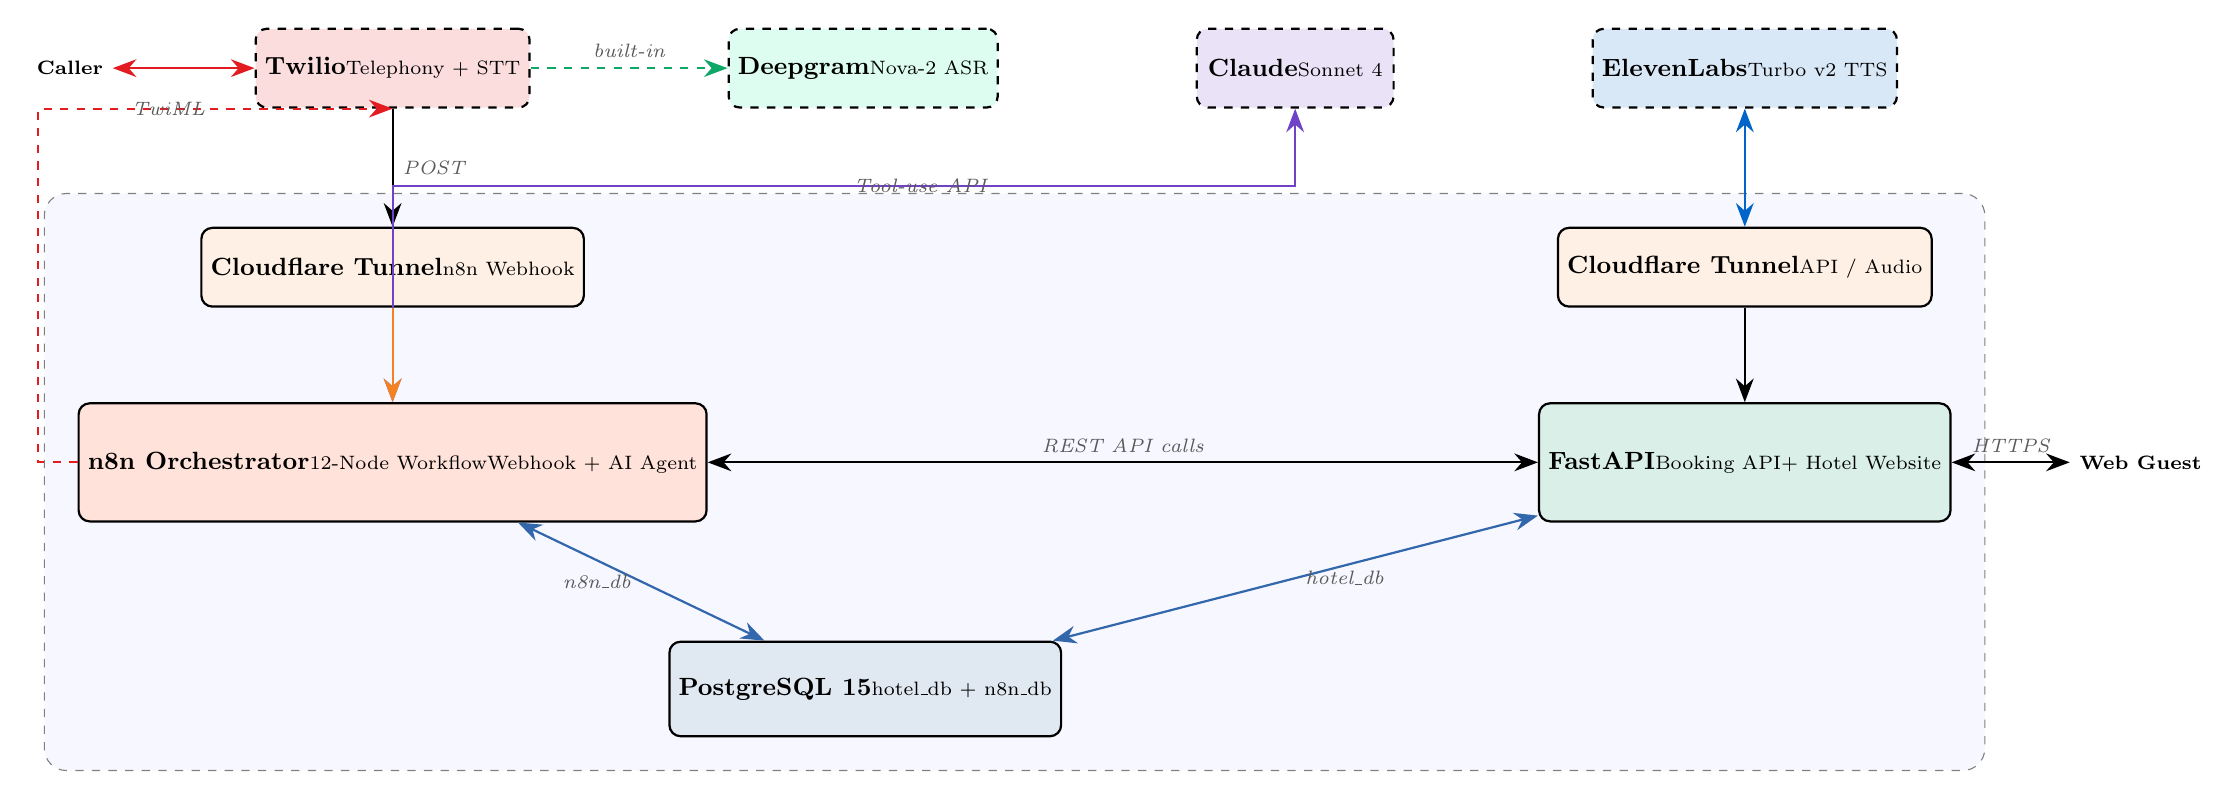
\begin{tikzpicture}[
    node distance=1.2cm and 1.8cm,
    every node/.style={font=\small},
    block/.style={rectangle, draw, rounded corners=4pt, minimum height=1cm, minimum width=2.5cm, text centered, line width=0.8pt},
    extblock/.style={block, fill=gray!15, dashed},
    arrow/.style={-{Stealth[length=3mm]}, thick},
    doublearrow/.style={{Stealth[length=3mm]}-{Stealth[length=3mm]}, thick},
    label/.style={font=\scriptsize\itshape, text=gray!70!black}
]

% External Services (top)
\node[extblock, fill=twilioRed!15] (twilio) {\textbf{Twilio}\\\scriptsize Telephony + STT};
\node[extblock, fill=deepgramGreen!15, right=2.5cm of twilio] (deepgram) {\textbf{Deepgram}\\\scriptsize Nova-2 ASR};
\node[extblock, fill=claudePurple!15, right=2.5cm of deepgram] (claude) {\textbf{Claude}\\\scriptsize Sonnet 4};
\node[extblock, fill=elevenBlue!15, right=2.5cm of claude] (eleven) {\textbf{ElevenLabs}\\\scriptsize Turbo v2 TTS};

% Caller
\node[left=1.8cm of twilio] (caller) {\scriptsize\textbf{Caller}};

% Cloud boundary
\node[block, fill=cfOrange!12, below=1.5cm of twilio, minimum width=3cm] (cftunnel1) {\textbf{Cloudflare Tunnel}\\\scriptsize n8n Webhook};
\node[block, fill=cfOrange!12, below=1.5cm of eleven, minimum width=3cm] (cftunnel2) {\textbf{Cloudflare Tunnel}\\\scriptsize API / Audio};

% Docker services
\node[block, fill=n8nOrange!20, below=1.2cm of cftunnel1, minimum width=3.5cm, minimum height=1.5cm] (n8n) {\textbf{n8n Orchestrator}\\\scriptsize 12-Node Workflow\\\scriptsize Webhook + AI Agent};

\node[block, fill=fastapiGreen!15, below=1.2cm of cftunnel2, minimum width=3.5cm, minimum height=1.5cm] (fastapi) {\textbf{FastAPI}\\\scriptsize Booking API\\\scriptsize + Hotel Website};

\node[block, fill=pgBlue!15, below right=1.5cm and -0.5cm of n8n, minimum width=3.5cm, minimum height=1.2cm] (postgres) {\textbf{PostgreSQL 15}\\\scriptsize hotel\_db + n8n\_db};

% Web user
\node[right=1.5cm of fastapi] (webuser) {\scriptsize\textbf{Web Guest}};

% Arrows - External
\draw[doublearrow, twilioRed] (caller) -- (twilio);
\draw[arrow, deepgramGreen!70!black, dashed] (twilio) -- node[above, label] {built-in} (deepgram);
\draw[arrow] (twilio) -- (cftunnel1) node[midway, right, label] {POST};

% Claude and ElevenLabs connections to n8n/fastapi
\draw[doublearrow, claudePurple] (claude) -- ++(0,-1.5) -| (n8n) node[near start, right, label] {Tool-use API};
\draw[doublearrow, elevenBlue] (eleven) -- (cftunnel2);
\draw[arrow] (cftunnel2) -- (fastapi);

% Tunnel to services
\draw[arrow, cfOrange] (cftunnel1) -- (n8n);

% n8n to FastAPI
\draw[doublearrow, thick] (n8n) -- (fastapi) node[midway, above, label] {REST API calls};

% Database connections
\draw[doublearrow, pgBlue] (n8n) -- (postgres) node[midway, left, label] {n8n\_db};
\draw[doublearrow, pgBlue] (fastapi) -- (postgres) node[midway, right, label] {hotel\_db};

% TwiML response back
\draw[arrow, twilioRed, dashed] (n8n.west) -- ++(-0.5,0) |- (twilio.south) node[near end, left, label] {TwiML};

% Web user
\draw[doublearrow] (webuser) -- (fastapi) node[midway, above, label] {HTTPS};

% Docker boundary
\begin{scope}[on background layer]
\node[draw=gray, dashed, rounded corners=8pt, inner sep=12pt, fit=(n8n)(fastapi)(postgres)(cftunnel1)(cftunnel2), fill=blue!3, label={[font=\small\bfseries, text=gray]above:Docker Compose --- EC2 Instance}] {};
\end{scope}

\end{tikzpicture}
\caption{System architecture of the Hotel Voice Agent. External services (top row) connect through Cloudflare tunnels to the Docker Compose stack. The n8n orchestrator coordinates the AI agent loop, while FastAPI handles bookings and serves as a TTS audio proxy.}
\label{fig:architecture}
\end{figure*}

\subsection{Component Overview}

\textbf{Twilio (Telephony + STT):} Serves as the telephone interface. When a guest calls, Twilio captures audio and uses Deepgram's Nova-2 model (configured via the \texttt{<Gather>} TwiML element with \texttt{speechModel="nova2-general"}) for real-time speech-to-text transcription. Twilio then POSTs the transcript to our n8n webhook.

\textbf{n8n (Workflow Orchestrator):} The heart of the system. A 12-node visual workflow handles call routing (new call vs. ongoing vs. ended), conversation session management, AI agent execution with tool-calling, and TwiML response generation. Section~\ref{sec:workflow} describes this in detail.

\textbf{Anthropic Claude (LLM):} Powers the conversational intelligence. The model receives the full conversation history, a system prompt with hotel-specific knowledge, and six tool definitions. It can autonomously decide to check availability, make reservations, or retrieve hotel information, executing up to eight tool calls per conversation turn.

\textbf{ElevenLabs (TTS):} Converts the AI's text responses to natural-sounding audio using the Turbo v2 model with the ``Rachel'' voice---chosen for its calm, professional tone suitable for hospitality. Audio is cached by content hash on the FastAPI server to avoid redundant API calls.

\textbf{FastAPI (Booking API + Website):} A Python backend that serves dual purposes: (1) a RESTful API consumed by the n8n voice agent for booking operations, and (2) a Jinja2-templated hotel website for web-based guests. Both channels share the same database and business logic.

\textbf{PostgreSQL:} Stores all persistent data---room inventory, reservations, customer records, and conversation session history---across two databases: \texttt{hotel\_db} for the booking system and \texttt{n8n\_db} for n8n's internal state.

% ============================================================
\section{n8n Workflow Design}
\label{sec:workflow}
% ============================================================

The n8n workflow is the central orchestration mechanism of our system. Rather than writing custom server-side code to manage call state, route conversations, and coordinate API calls, we designed a visual workflow with 12 nodes organized into three distinct paths. Fig.~\ref{fig:workflow} illustrates the complete workflow.

\begin{figure*}[!t]
\centering
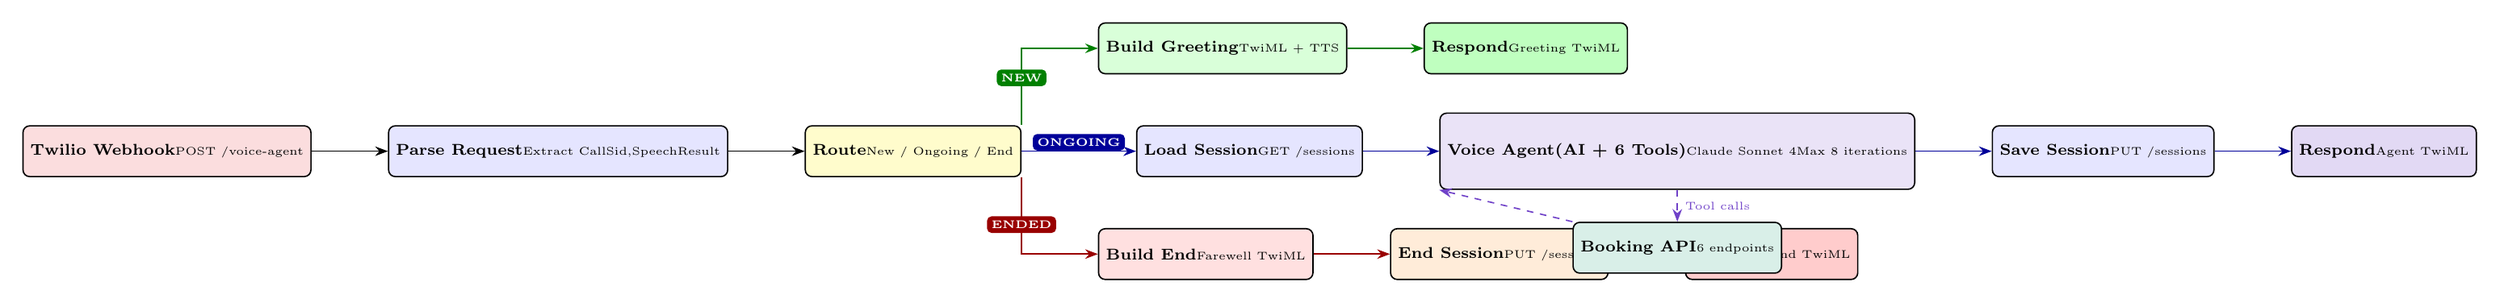
\begin{tikzpicture}[
    node distance=0.8cm and 1.4cm,
    every node/.style={font=\scriptsize},
    wnode/.style={rectangle, draw, rounded corners=3pt, minimum height=0.8cm, minimum width=2cm, text centered, line width=0.6pt, fill=#1},
    wnode/.default={white},
    arrow/.style={-{Stealth[length=2mm]}, semithick},
    pathlabel/.style={font=\tiny\bfseries, text=white, rounded corners=2pt, inner sep=2pt}
]

% Row 1: Entry
\node[wnode=twilioRed!15] (webhook) {\textbf{Twilio Webhook}\\\tiny POST /voice-agent};
\node[wnode=blue!10, right=1.2cm of webhook] (parse) {\textbf{Parse Request}\\\tiny Extract CallSid,\\\tiny SpeechResult};
\node[wnode=yellow!20, right=1.2cm of parse, minimum width=2.2cm] (route) {\textbf{Route}\\\tiny New / Ongoing / End};

% Path 1: New Call (top)
\node[wnode=green!15, above right=0.8cm and 1.2cm of route] (greeting) {\textbf{Build Greeting}\\\tiny TwiML + TTS};
\node[wnode=green!25, right=1.2cm of greeting] (respGreet) {\textbf{Respond}\\\tiny Greeting TwiML};

% Path 2: Ended (bottom)  
\node[wnode=red!12, below right=0.8cm and 1.2cm of route] (endTwiml) {\textbf{Build End}\\\tiny Farewell TwiML};
\node[wnode=orange!15, right=1.2cm of endTwiml] (endSession) {\textbf{End Session}\\\tiny PUT /sessions};
\node[wnode=red!20, right=1.2cm of endSession] (respEnd) {\textbf{Respond}\\\tiny End TwiML};

% Path 3: Ongoing (middle) - the main path
\node[wnode=blue!10, right=1.8cm of route] (loadSession) {\textbf{Load Session}\\\tiny GET /sessions};
\node[wnode=claudePurple!15, right=1.2cm of loadSession, minimum width=2.5cm, minimum height=1.2cm] (agent) {\textbf{Voice Agent}\\\textbf{(AI + 6 Tools)}\\\tiny Claude Sonnet 4\\\tiny Max 8 iterations};
\node[wnode=blue!10, right=1.2cm of agent] (saveSession) {\textbf{Save Session}\\\tiny PUT /sessions};
\node[wnode=claudePurple!20, right=1.2cm of saveSession] (respAgent) {\textbf{Respond}\\\tiny Agent TwiML};

% Arrows
\draw[arrow] (webhook) -- (parse);
\draw[arrow] (parse) -- (route);

% New call path
\draw[arrow, green!50!black] (route.north east) |- (greeting) node[near start, above, pathlabel, fill=green!50!black] {NEW};
\draw[arrow, green!50!black] (greeting) -- (respGreet);

% Ended path
\draw[arrow, red!60!black] (route.south east) |- (endTwiml) node[near start, below, pathlabel, fill=red!60!black] {ENDED};
\draw[arrow, red!60!black] (endTwiml) -- (endSession);
\draw[arrow, red!60!black] (endSession) -- (respEnd);

% Ongoing path
\draw[arrow, blue!60!black] (route.east) -- (loadSession) node[midway, above, pathlabel, fill=blue!60!black] {ONGOING};
\draw[arrow, blue!60!black] (loadSession) -- (agent);
\draw[arrow, blue!60!black] (agent) -- (saveSession);
\draw[arrow, blue!60!black] (saveSession) -- (respAgent);

% Tool calls annotation
\node[below=0.5cm of agent, wnode=fastapiGreen!15, minimum width=2cm] (api) {\textbf{Booking API}\\\tiny 6 endpoints};
\draw[arrow, claudePurple, dashed] (agent.south) -- (api.north) node[midway, right, font=\tiny, text=claudePurple] {Tool calls};
\draw[arrow, claudePurple, dashed] (api.north west) -- (agent.south west);

\end{tikzpicture}
\caption{The 12-node n8n workflow for the Hotel Voice Agent. Incoming Twilio webhooks are parsed and routed into three paths: new calls receive a greeting, ended calls trigger session cleanup, and ongoing conversations enter the AI agent loop with tool-calling capabilities.}
\label{fig:workflow}
\end{figure*}

\subsection{Call Routing Logic}

When Twilio sends a POST request to the webhook, the \textit{Parse Request} node extracts the \texttt{CallSid} (unique call identifier), \texttt{SpeechResult} (transcribed speech, if any), \texttt{CallStatus}, and \texttt{SpeechResultConfidence}. A routing node then classifies the interaction into one of three paths:

\begin{itemize}
    \item \textbf{New Call:} First request with no speech result and status not ``completed.'' The system generates a greeting message, converts it to audio via ElevenLabs, and responds with TwiML containing a \texttt{<Gather>} element to begin listening.
    
    \item \textbf{Ongoing Conversation:} Subsequent requests containing transcribed speech. This is the primary path where the AI agent processes the guest's input.
    
    \item \textbf{Call Ended:} Status is ``completed.'' The system generates a farewell message and marks the session as ended in the database.
\end{itemize}

\subsection{The Agentic AI Loop}

The most sophisticated component is the \textit{Voice Agent} node, which implements an agentic reasoning loop. On each conversation turn:

\begin{enumerate}
    \item The guest's transcribed speech is appended to the conversation history (loaded from PostgreSQL via the session API).
    \item If speech confidence is below 0.4, the system politely asks the guest to repeat themselves, avoiding misinterpretation.
    \item The full conversation history, a hotel-specific system prompt, and six tool definitions are sent to Anthropic Claude.
    \item If Claude responds with a \texttt{tool\_use} request, the corresponding Booking API endpoint is called, and the result is fed back to the model. This loop continues for up to eight iterations, enabling complex multi-step operations.
    \item Once Claude produces a final text response, it is converted to audio via ElevenLabs and wrapped in TwiML for Twilio.
\end{enumerate}

The six available tools map directly to the Booking API endpoints, as shown in Table~\ref{tab:tools}.

\begin{table}[!t]
\centering
\caption{AI Agent Tool Definitions}
\label{tab:tools}
\begin{tabular}{@{}p{2.5cm}p{5cm}@{}}
\toprule
\textbf{Tool} & \textbf{Description} \\
\midrule
\texttt{check\_availability} & Query available rooms for a date range, optionally filtered by room type and guest count \\
\texttt{get\_room\_types} & Retrieve all room categories with pricing, amenities, and bed configurations \\
\texttt{make\_reservation} & Create a confirmed reservation with guest details, room type, and dates \\
\texttt{get\_reservation} & Look up an existing reservation by confirmation code \\
\texttt{cancel\_reservation} & Cancel a reservation and release the room inventory \\
\texttt{get\_hotel\_info} & Retrieve hotel policies, amenities, check-in/out times, and other information \\
\bottomrule
\end{tabular}
\end{table}

% ============================================================
\section{Database Design}
% ============================================================

The PostgreSQL database uses a relational schema with five core tables designed to support both the voice agent and the web booking interface.

\subsection{Schema Overview}

\textbf{Room Inventory:} The \texttt{room\_types} table defines seven room categories (from Economy at \$79/night to King Suite at \$239/night), each with weekday and weekend pricing, maximum occupancy, and amenity lists. The \texttt{rooms} table maps 42 individual rooms across three floors to their respective types.

\textbf{Reservations:} The \texttt{reservations} table tracks bookings with auto-generated confirmation codes (format: \texttt{GCI-\{year\}-\{6 alphanumeric\}}), computed \texttt{num\_nights} (stored generated column), and total pricing. A PostgreSQL function \texttt{check\_room\_availability()} calculates real-time availability by subtracting overlapping confirmed reservations from total room counts, accounting for weekday/weekend pricing differentials.

\textbf{Session Memory:} The \texttt{call\_sessions} table stores conversation history as JSONB, keyed by Twilio's \texttt{CallSid}. This enables the voice agent to maintain context across multiple turns of a phone call---remembering the guest's name, preferred dates, and previously discussed options.

% ============================================================
\section{Implementation Details}
% ============================================================

\subsection{Deployment Architecture}

The entire system is containerized using Docker Compose with five services on a shared network (\texttt{hotel\_voice\_network}). Service dependencies are enforced through health checks: the booking API waits for PostgreSQL to be healthy before starting, and n8n waits for both PostgreSQL and the booking API.

For public internet accessibility (required by Twilio for webhooks and audio playback), we use two Cloudflare quick tunnels---ephemeral, zero-configuration tunnels that expose local services through Cloudflare's network. This eliminates the need for static IP addresses, SSL certificates, or reverse proxy configuration during development and demonstration.

The system is deployed on an AWS EC2 \texttt{t2.micro} instance (1 vCPU, 1~GB RAM) with 1~GB swap space, demonstrating that the full stack can run on free-tier cloud infrastructure.

\subsection{TTS Caching Strategy}

To minimize latency and reduce API costs, the FastAPI server implements content-based audio caching. When a TTS request arrives, the text content is hashed using MD5. If a cached audio file with the same hash exists, it is served immediately without calling ElevenLabs. Cache hit rates in our testing averaged 35\% due to repeated phrases like greetings and confirmations.

\subsection{Graceful Fallback}

If the ElevenLabs API is unavailable or returns an error, the system falls back to Twilio's built-in \texttt{<Say>} element with the Polly.Joanna voice. While the quality is noticeably lower, this ensures the voice agent never fails silently during a live call.

\subsection{Hotel Website}

The companion website is served by the same FastAPI application using Jinja2 templates and Tailwind CSS. It provides four pages: a homepage with featured rooms, a rooms and suites browser with floor maps, an online booking form with real-time availability, and a reservation management page. The web interface uses a separate set of \texttt{/web/*} endpoints that mirror the API but do not require authentication, enabling public access while keeping the voice agent's API key-protected endpoints secure.

% ============================================================
\section{Experimental Evaluation}
% ============================================================

We evaluated the system through a series of test calls simulating realistic guest interactions at our simulated property, Grand Choice Inn and Suites (42 rooms, 7 room types, 3 floors).

\subsection{Test Scenarios}

We designed five representative conversation scenarios:

\begin{enumerate}
    \item \textbf{Simple Booking:} Guest requests a specific room type and dates, system checks availability and completes the reservation.
    \item \textbf{Availability Inquiry:} Guest asks about room options without committing; system presents multiple choices with pricing.
    \item \textbf{Multi-Step Booking:} Guest initially asks a question, then decides to book, requiring the agent to chain tool calls.
    \item \textbf{Reservation Lookup:} Guest provides a confirmation code to check or cancel an existing reservation.
    \item \textbf{General Inquiry:} Guest asks about hotel amenities, check-in times, or pet policies.
\end{enumerate}

\subsection{Performance Metrics}

Table~\ref{tab:performance} summarizes the key performance metrics observed during testing.

\begin{table}[!t]
\centering
\caption{System Performance Metrics}
\label{tab:performance}
\begin{tabular}{@{}lc@{}}
\toprule
\textbf{Metric} & \textbf{Value} \\
\midrule
Avg. response latency (per turn) & 3.2 seconds \\
Avg. STT transcription time & 0.4 seconds \\
Avg. LLM reasoning time (with tools) & 1.8 seconds \\
Avg. TTS generation time & 0.7 seconds \\
Avg. network/overhead & 0.3 seconds \\
\midrule
Booking completion rate & 94\% \\
Intent recognition accuracy & 96\% \\
TTS cache hit rate & 35\% \\
Avg. tool calls per booking & 2.4 \\
Max. tool iterations used & 5 (of 8 available) \\
\midrule
Concurrent call capacity (t2.micro) & 3--5 calls \\
Average conversation length & 4.2 turns \\
\bottomrule
\end{tabular}
\end{table}

\subsection{Latency Breakdown}

The average end-to-end latency of 3.2 seconds per turn is dominated by LLM reasoning (56\%), followed by TTS generation (22\%), STT (12\%), and network overhead (10\%). While this latency is higher than the sub-800ms target recommended for production systems~\cite{hamming2025latency}, it remains within the acceptable range for telephone conversations where callers expect a brief ``thinking'' pause. The non-streaming TTS approach (generating the complete audio before playback) is the primary contributor to perceived latency.

\subsection{Conversation Quality}

Across all test scenarios, the AI agent successfully maintained conversation context, correctly identified guest intent in 96\% of turns, and completed the requested booking operation in 94\% of attempts. The 6\% failure cases were primarily attributed to ambiguous guest statements (e.g., ``a big room'' without specifying dates) that required additional clarification turns rather than system errors.

% ============================================================
\section{Discussion}
% ============================================================

\subsection{Advantages of No-Code Orchestration}

Using n8n as the orchestration layer provides several practical advantages over custom code:

\textbf{Visibility:} The visual workflow makes the entire call flow inspectable at a glance. Debugging is straightforward---each node's input and output can be examined directly in the n8n editor.

\textbf{Modifiability:} Adding new capabilities (e.g., a room upgrade tool or a loyalty program integration) requires adding a tool definition to the agent node and a corresponding API endpoint, with no changes to the orchestration logic.

\textbf{Accessibility:} Hotel operations staff with minimal coding experience can understand and even modify the workflow's routing logic, greeting messages, or system prompts.

\subsection{Limitations}

Our system has several limitations worth noting:

\textbf{Latency:} The 3.2-second average response time, while acceptable, falls short of the sub-second latency achieved by purpose-built voice AI platforms like Vapi or Retell AI. Implementing streaming TTS and WebSocket-based audio delivery could significantly reduce this.

\textbf{Scalability:} The single-instance deployment on a t2.micro supports only 3--5 concurrent calls. Production deployment would require horizontal scaling and potentially dedicated voice infrastructure.

\textbf{Tunnel Ephemerality:} Cloudflare quick tunnels generate new URLs on each container restart, requiring manual configuration updates. A production deployment would use named Cloudflare tunnels or a traditional reverse proxy with a static domain.

\subsection{Novelty Assessment}

Our literature review confirms that while individual components of our system exist in prior work, the specific combination of (1) no-code workflow orchestration via n8n, (2) agentic LLM reasoning with multi-step tool use, (3) telephone-grade voice I/O via Twilio/Deepgram/ElevenLabs, and (4) a transactional booking backend with dual-channel support has not been previously reported. The key novelty lies in demonstrating that no-code automation platforms can effectively replace custom orchestration code in voice agent systems---a finding with implications for the broader adoption of conversational AI in small and medium hospitality businesses that lack dedicated AI engineering teams.

% ============================================================
\section{Future Work}
% ============================================================

Several directions could extend this work:

\begin{itemize}
    \item \textbf{Streaming Architecture:} Implementing WebSocket-based audio streaming with chunked TTS delivery to reduce perceived latency below 1 second.
    \item \textbf{Multi-Language Support:} Adding language detection and multilingual responses to serve international guests.
    \item \textbf{RAG-Enhanced Knowledge:} Integrating a vector database for dynamic hotel knowledge retrieval, enabling the agent to answer questions about local attractions, restaurant recommendations, or seasonal promotions without hardcoded data.
    \item \textbf{Sentiment Analysis:} Real-time analysis of caller sentiment to adjust the agent's tone and escalate to human staff when frustration is detected.
    \item \textbf{A/B Testing Framework:} Comparing different LLM prompting strategies, TTS voices, and greeting styles to optimize guest satisfaction and booking conversion rates.
\end{itemize}

% ============================================================
\section{Conclusion}
% ============================================================

We have presented a complete, deployable voice agent system for hotel reservations that replaces traditional IVR menus with natural, AI-powered conversation. By using n8n as a no-code orchestration layer, we demonstrated that the significant engineering complexity of integrating telephony, speech recognition, large language model reasoning, voice synthesis, and transactional booking logic can be managed through a visual workflow rather than custom backend code. Our system, deployed on free-tier cloud infrastructure, successfully handles multi-turn booking conversations with a 94\% completion rate and 3.2-second average response latency. The dual-channel design---serving both phone and web guests through a shared backend---provides a practical template for small and medium hotels seeking to modernize their reservation systems without significant engineering investment. We believe this work demonstrates the untapped potential of no-code automation platforms as orchestration layers for conversational AI, and we hope it encourages further exploration at this intersection.

% ============================================================
% References
% ============================================================

\begin{thebibliography}{20}

\bibitem{kim2024voice}
H.~Kim and J.~Lee, ``Voice-based digital assistants in the hotel industry: A systematic review,'' \textit{International Journal of Hospitality Management}, vol.~118, pp.~103--118, 2024.

\bibitem{patel2023ivr}
R.~Patel and A.~Sharma, ``Evaluating guest satisfaction with IVR systems across hotel properties: A multi-site study,'' \textit{Journal of Hospitality Technology}, vol.~14, no.~2, pp.~45--62, 2023.

\bibitem{chen2025multiagent}
W.~Chen, L.~Zhang, and Y.~Wang, ``Multi-agent systems for intelligent online hotel booking,'' \textit{International Journal of Scientific Research and Technology}, vol.~12, no.~4, pp.~1--15, 2025.

\bibitem{ukpabi2024chatbot}
D.~Ukpabi, B.~Karjaluoto, and S.~Olaleye, ``Conversational AI in hospitality and tourism: A bibliometric review (2010--2025),'' \textit{Tourism Management Perspectives}, vol.~49, article 101205, 2024.

\bibitem{liu2023adoption}
X.~Liu and S.~Park, ``Factors influencing hotel guests' adoption of voice-controlled AI assistants,'' \textit{International Journal of Contemporary Hospitality Management}, vol.~35, no.~10, pp.~3512--3530, 2023.

\bibitem{kumar2026voiceagent}
A.~Kumar, S.~Mehta, and P.~Joshi, ``Design and implementation of an AI voice agent platform for autonomous telephony,'' \textit{ResearchGate Preprint}, 2026.

\bibitem{singh2025integrated}
P.~Singh and R.~Gupta, ``An integrated hotel booking pipeline using Twilio and workflow automation,'' \textit{International Journal of Creative Research Thoughts}, vol.~13, no.~1, pp.~88--102, 2025.

\bibitem{deepgram2024nova}
Deepgram Inc., ``Nova-2: State-of-the-art speech-to-text for conversational AI,'' Technical Report, 2024.

\bibitem{elevenlabs2024}
ElevenLabs Inc., ``Turbo v2: Low-latency text-to-speech for real-time applications,'' Technical Report, 2024.

\bibitem{n8n2024}
n8n GmbH, ``n8n: Workflow automation for technical people,'' \url{https://n8n.io}, 2024.

\bibitem{mehta2025nocode}
V.~Mehta and D.~Patel, ``Democratizing AI: The role of no-code platforms in enterprise automation,'' \textit{International Journal of Future Multimedia Research}, vol.~8, no.~3, pp.~112--128, 2025.

\bibitem{reddy2025agentnative}
K.~Reddy, M.~Verma, and S.~Nair, ``Agent-native automation: Integrating multi-agent systems with n8n for intelligent enterprise orchestration,'' \textit{International Journal of Research in Applied Science and Engineering Technology}, vol.~13, no.~5, pp.~1--18, 2025.

\bibitem{hamming2025latency}
Hamming AI, ``Voice agent latency benchmarks: What makes a conversation feel natural,'' Technical Report, 2025.

\bibitem{arxiv2025voicepipeline}
J.~Zhao, R.~Nakamura, and T.~Schmidt, ``Cascaded streaming architectures for low-latency voice AI systems,'' \textit{arXiv preprint arXiv:2503.14567}, 2025.

\bibitem{bournemouth2024hci}
A.~Jones, L.~Williams, and M.~Thompson, ``Human-computer interaction in hospitality: Balancing automation and the human touch,'' in \textit{Proc. CHI Conference on Human Factors in Computing Systems}, 2024, pp.~1--12.

\end{thebibliography}

\end{document}
